%%% LaTeX Template: Article/Thesis/etc. with colored headings and special fonts
%%%
%%% Source: http://www.howtotex.com/

\documentclass[12pt]{article}


\usepackage{apuntes-estilo}
\usepackage{fancyhdr,lastpage}
\usepackage{color,colortbl}
\usepackage{verbatim}

\def\maketitle{

% Titulo 
 \makeatletter
 {\color{bl} \centering \huge \sc \textbf{
 Particionado y sistema de archivos \\ 
\large \vspace*{-8pt} \color{black} Guía básica sobre particionado y sistema de archivos.
 \vspace*{8pt} }\par}
 \makeatother


% Autor
 \makeatletter
 {\centering \small 
 	Departamento de Ingeniería de Computadoras \\
 	Facultad de Informática - Universidad Nacional del Comahue \\
 	\vspace{20pt} }
 \makeatother

}

% Custom headers and footers
\fancyhf{} % clear all header and footer fields
\fancypagestyle{plain}{\fancyhf{}}
  	\pagestyle{fancy}
 	\lhead{\footnotesize Particionado y sistema de archivos - Departamento de Ingeniería de Computadoras}
 	\rhead{\footnotesize \thepage\ }	% ''Page 1 of 2''

\def\ti#1#2{\texttt{#1} & #2 \\ }



\begin{document}

\thispagestyle{empty}
\maketitle
\setlength{\parindent}{0pt}

\section*{Introducción}

Las actividades sobre los medios masivos de almacenamiento son altamente 
frecuentes dentro de las tareas de los administradores. La administración 
del espacio de almacenamiento (datos), involucra varias tareas: diseño 
del uso de discos, particionado para ajustarse al diseño, creación de 
sistema de archivos que permitan organizar la información dentro de los
discos (que de por sí no son más que una secuencia de bits sin sentido),
monitoreo del consumo de espacio, ajustes de acuerdo al uso, copias de 
respaldo en caso de fallas, entre otras. 

En este apunte se cubren los conceptos básicos de particionamiento de 
discos y sistemas de archivos.  

\section*{Particiones}

Un disco rígido puede dividirse en varias particiones. {\bf Cada partición 
funciona como si fuera un disco duro independiente.} 
La idea es que si sólo se tiene un disco, y se quieren tener, digamos,
 dos sistemas operativos en él, se pueda dividir 
el disco en dos particiones. Cada sistema operativo utilizará su propia 
partición tal y como se desea, y no tocará 
la otra. De esta forma los dos sistemas operativos pueden coexistir 
pacíficamente en un mismo disco rígido. En este ejemplo, si no tuviésemos
particiones necesitaríamos comprar un disco rígido para cada sistema 
operativo.

Además de los discos rígidos, otros dispositivos de almacenamiento 
masivo suelen particionarse, como por ejemplo las memorias flash (pendrive).
Este apunte pretende cubrir el concepto de particionado, aplicando en 
particular dicho concepto a los esquemas seguidos por las PC convencionales.  


\subsection*{El MBR, sectores de arranque y la tabla de particiones}

La información sobre cómo se particiona un disco se almacena en su primer 
sector (estos son los primeros bytes al comienzo del dispositivo, 
dependiendo del tipo de dispositivo particular es la cantidad de bytes 
que representan el primer sector). Este primer sector es el registro de 
arranque maestro (MBR, del inglés Master Boot Record) del disco; éste es 
el sector que la BIOS lee y arranca cuando se enciende la máquina. 

El esquema de partición no está integrado en el hardware, ni siquiera 
en la BIOS. Tan sólo es una convención que muchos (no todos) sistemas 
operativos siguen. Algunos sistemas operativos soportan particiones pero 
con esquemas diferentes, en muchos casos para coexistir con el esquema 
mencionado, ocupan una partición convencional en el disco duro, y 
utilizan su propio sistema de particionamiento dentro de esa partición 
(por ejemplo, esto sucede con el sistema operativo Solaris sobre 
arquitectura x86). La mayoría de los sistemas operativos modernos
soportan particionado, sin embargo es bueno tener presente que si estamos 
frente a un sistema operativo  que no lo soporta, entonces  no podrá 
coexistir en un mismo disco con los que si. 

Es importante almacenar la información detallada de las tablas de 
particiones en una computadora distinta, mediante algún mecanismo de 
copia de respaldo, para poder recuperar la información almacenada en 
caso de que la tabla de particiones sea modificada por error. En 
particular el comando \texttt{fdisk} nos permite listar esta información: 

\colorbox{grey}{\parbox[t]{0.95\linewidth}{ \vspace*{0.5cm} { 
{\bf Ejemplo : información de particiones del disco \texttt{/dev/sdb}}\\
{\tt
\#fdisk -l /dev/sdb\\
Disk /dev/sdb: 80.0 GB, 80032038912 bytes\\
255 heads, 63 sectors/track, 9730 cylinders, 156312576 sectores en total\\
Units = sectores of 1 * 512 = 512 bytes\\
Sector size (logical/physical): 512 bytes / 512 bytes\\
I/O size (minimum/optimal): 512 bytes / 512 bytes\\
Identificador del disco: 0x00005700\\
\\
Disposit. Inicio    Comienzo      Fin      Bloques  Id  Sistema\\
/dev/sdb1   *        2048    39063551    19530752   83  GNU/Linux\\
/dev/sdb2        39063552    42969087     1952768   82  GNU/Linux swap / Solaris\\
/dev/sdb3        42969088   156311551    56671232   83  GNU/Linux\\
}
} \vspace*{0.5cm} } } 

\subsection*{Particiones extendidas y lógicas}

El esquema original de particionamiento para discos duros de PC permitía 
solamente cuatro particiones. Esto rápidamente se volvió demasiado escaso 
para la vida real, en parte porque algunas personas querían más de cuatro 
sistemas operativos (Linux, MS-DOS, OS/2, Minix, FreeBSD, NetBSD, o 
Windows/NT, por nombrar algunos), pero principalmente 
porque algunas veces es buena idea tener varias particiones para un mismo 
sistema operativo. Por ejemplo, el espacio swap está generalmente mejor 
colocado para GNU/Linux en su propia partición en lugar de la partición 
principal por cuestiones de rapidez (vea más abajo). También por ejemplo 
podríamos querer limitar el espacio disponible 
para archivos de usuarios, de modo que el directorio \texttt{/home} se 
encuentre en una partición separada. 

Para superar esta limitación de diseño, se inventaron las particiones 
extendidas. Este truco permite particionar una partición primaria en 
sub-particiones. Esta partición primaria subdividida es la partición 
extendida; las sub-particiones son las particiones lógicas. Se comportan 
como particiones primarias, pero se crean de diferente manera. No existen
diferencias de rendimiento entre ellas.

La estructura de particiones de un disco duro debe parecerse a la que 
aparece en la figura a continuación. El disco se divide en tres particiones 
primarias, la segunda de las cuales se divide en dos 
particiones lógicas. Una parte del disco no está particionada. El disco 
como un todo y cada partición primaria tienen un sector de arranque.

\begin{center}
 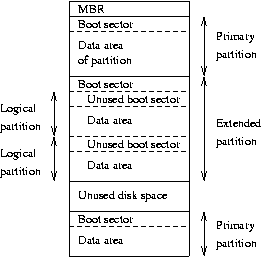
\includegraphics{hd-layout.png}
\end{center}

\subsection*{Particionando el disco duro}

Existen muchos programas para crear y eliminar particiones. La mayoría de 
sistemas operativos tienen el suyo propio, y es buena idea utilizar el 
propio con cada sistema operativo, por si se diera el caso que haga algo 
inusual que los otros no puedan hacer. Muchos de estos programas se 
llaman \texttt{fdisk}, incluido el de GNU/Linux, o variaciones de esa 
palabra. Los detalles de uso del fdisk de GNU/Linux se dan en su página 
de manual. El comando \texttt{cfdisk} es similar a \texttt{fdisk}, pero tiene 
una interfaz más sencilla para usuarios no familiarizados con el 
particionado. Existen programas gráficos, como los utilizados por los 
instaladores de la distribución Ubuntu, sin embargo alentamos a los 
lectores a utilizar \texttt{fdisk} por estar también disponible en 
otros sistemas UNIX y ser el comando por excelencia utilizado por 
administradores de sistemas. 

Cambiar el tamaño de una partición es una actividad que puede involucrar
pérdida de datos, en caso de discos con información preexistente al 
momento de particionar. Por lo que requiere que primero se realice una 
copia de respaldo de todo lo que se quiera preservar de la partición en 
cuestión (a ser posible de todo el disco, por si acaso), borrar la 
partición, crear una nueva, y entonces restaurar los datos a la nueva 
partición. Esto puede suceder si los datos almacenados han crecido más de 
lo esperado y se hace necesario re-estructar las particiones en el disco 
para ajustarse a la nueva demanda. 

\fcolorbox{black}{grey}{
\parbox[t]{1.0\linewidth}{ \vspace*{0.4cm}
{\bf Lo importante:} cambiar una partición es complejo y riesgoso,  por lo 
que es recomendable hacer una evaluación concienzuda al momento de crearlas,
y contar con buenas herramientas de copia de respaldo.   
\vspace*{0.4cm} } }

{\bf Ejemplo de secuencia de creación de particiones utilizando
\texttt{fdisk} sobre el disco /dev/sdc}

{\tt
\# fdisk /dev/sdc\\
\\
\textbf{... listamos la tabla de particiones actual ...}\\
\\
Orden (m para obtener ayuda):  {\bf p}\\
\\
Disco /dev/sdc: 4007 MB, 4007657472 bytes\\
124 heads, 62 sectors/track, 1018 cylinders, 7827456 sectores en total\\
Units = sectores of 1 * 512 = 512 bytes\\
Sector size (logical/physical): 512 bytes / 512 bytes\\
I/O size (minimum/optimal): 512 bytes / 512 bytes\\
Identificador del disco: 0x0006c58a\\
\\
Disposit. Inicio    Comienzo      Fin      Bloques  Id  Sistema\\
\\
\textbf{... creamos una nueva partición primaria ...}\\
\\
Orden (m para obtener ayuda):  {\bf n}\\
Partition type:\\
   p   primary (0 primary, 0 extended, 4 free)\\
   e   extended\\
Select (default p): p\\
Número de partición (1-4, valor predeterminado 1): \\
Se está utilizando el valor predeterminado 1\\
Primer sector (2048-7827455, valor predeterminado 2048): \\
Se está utilizando el valor predeterminado 2048\\
Last sector, +sectores or +size{K,M,G} (2048-7827455, valor predeterminado 7827455): +500M\\
\\
\textbf{... creamos una nueva partición extendida ...}\\
\\
Orden (m para obtener ayuda):  {\bf n}\\
Partition type:\\
   p   primary (1 primary, 0 extended, 3 free)\\
   e   extended\\
Select (default p): e\\
Número de partición (1-4, valor predeterminado 2): 2\\
Primer sector (1026048-7827455, valor predeterminado 1026048): \\
Se está utilizando el valor predeterminado 1026048\\
Last sector, +sectores or +size{K,M,G} (1026048-7827455, valor predeterminado 7827455): \\
Se está utilizando el valor predeterminado 7827455\\
\\
\textbf{... creamos una nueva partición lógica ...}\\
\\
Orden (m para obtener ayuda):  {\bf n}\\
Partition type:\\
   p   primary (1 primary, 1 extended, 2 free)\\
   l   logical (numbered from 5)\\
Select (default p): l\\
Adding logical partition 5\\
Primer sector (1028096-7827455, valor predeterminado 1028096): \\
Se está utilizando el valor predeterminado 1028096\\
Last sector, +sectores or +size{K,M,G} (1028096-7827455, valor predeterminado 7827455): +800M\\
\\
\textbf{... creamos una nueva partición lógica ...}\\
\\
Orden (m para obtener ayuda):  {\bf n}\\
Partition type:\\
   p   primary (1 primary, 1 extended, 2 free)\\
   l   logical (numbered from 5)\\
Select (default p): l\\
Adding logical partition 6\\
Primer sector (2668544-7827455, valor predeterminado 2668544): \\
Se está utilizando el valor predeterminado 2668544\\
Last sector, +sectores or +size{K,M,G} (2668544-7827455, valor predeterminado 7827455): \\
Se está utilizando el valor predeterminado 7827455\\
\\
\textbf{... listamos la nueva tabla de particiones, aún no guardamos\\
los cambios ...}\\
\\
Orden (m para obtener ayuda):  {\bf p}\\
\\
Disco /dev/sdc: 4007 MB, 4007657472 bytes\\
124 heads, 62 sectors/track, 1018 cylinders, 7827456 sectores en total\\
Units = sectores of 1 * 512 = 512 bytes\\
Sector size (logical/physical): 512 bytes / 512 bytes\\
I/O size (minimum/optimal): 512 bytes / 512 bytes\\
Identificador del disco: 0x0006c58a\\
\\
Disposit. Inicio    Comienzo      Fin      Bloques  Id  Sistema\\
/dev/sdc1            2048     1026047      512000   83  Linux\\
/dev/sdc2         1026048     7827455     3400704    5  Extendida\\
/dev/sdc5         1028096     2666495      819200   83  Linux\\
/dev/sdc6         2668544     7827455     2579456   83  Linux\\
\\
\textbf{... guardamos la nueva tabla en el disco  ...}\\
Orden (m para obtener ayuda): {\bf w}\\
¡Se ha modificado la tabla de particiones!\\
\\
Llamando a ioctl() para volver a leer la tabla de particiones.\\
Se están sincronizando los discos.\\
}

\subsection*{Archivos de dispositivo y particiones}

Cada partición y partición extendida posee su propio archivo de 
dispositivo. El convenio de nombres para estos archivos es que se añade 
un número de partición detrás del nombre del disco entero, con el 
convenio de que las particiones primarias van del 1 al 4 
(independientemente de cuantas particiones primarias existan) y las 
particiones lógicas tienen números mayores que 5 
(independientemente de la partición primaria en la que residan). Por 
ejemplo, \texttt{/dev/sda1} es la primera partición primaria del primer
disco duro, mientras que \texttt{/dev/sda5} será la primer partición 
lógica del mismo disco.

\section*{Sistemas de archivos}

Un disco y sus particiones por en si mismas no son más que una organización
de bits sin sentido. El administrador de sistemas definirá estructuras 
lógicas dentro de los discos y particiones que permitan dar sentido a esa
secuencia de bits, estos son los sistemas de archivos. 

En la gran mayoría de los casos, las aplicaciones que utilizamos hacen uso 
de estos sistemas de archivos para recuperar o almacenar datos en los 
discos. Por ejemplo cuando descargamos un archivo de la web a través de 
nuestro navegador, éste almacena el archivo descargado dentro de un 
sistema de archivos, es decir no usa los bits crudos (raw) del disco, sino 
que utiliza el sistema de archivos para ésta función. Si bien hay 
aplicaciones que organizan e interpretan los datos en disco directamente, 
sin un sistema de archivos como intermediario, esto es el caso menos 
frecuente. En este caso se dice que la aplicación usa los discos en crudo 
(en inglés, raw access). 

\subsection*{¿Qué son los sistemas de archivos?}

Un sistema de archivos son los métodos y estructuras de datos que un 
sistema operativo utiliza para seguir la pista de los archivos dentro de 
un disco o partición; es decir, es la manera en la que se organizan los 
archivos en el disco. El término también es utilizado para referirse a una
partición o disco que se está utilizando para almacenamiento, o el tipo del
sistema de archivos que utiliza. Así uno puede decir ``tengo dos sistemas 
de archivo'' refiriéndose a que tiene dos particiones en las que almacenar
archivos, o que uno utiliza el sistema de ``archivos extendido'', 
refiriéndose al tipo del sistema de archivos.

La diferencia entre un disco o partición y el sistema de archivos que 
contiene es importante. Unos pocos programas (incluyendo, razonablemente, 
aquellos que crean sistemas de archivos) trabajan directamente en los 
sectores crudos del disco o partición. La mayoría de 
programas trabajan sobre un sistema de archivos, y por lo tanto no 
utilizarán una partición que no contenga uno (o que contenga uno del tipo 
equivocado).

Antes de que una partición o disco sea utilizada como un sistema de 
archivos, necesita ser iniciada, y las estructura de datos necesitan 
escribirse al disco. Este proceso se denomina \textbf{construir un sistema
de archivos}.

Si bien no es la intención de este apunte ahondar en los detalles de 
implementación de los sistemas de archivos, con la intención de que el 
lector se forme una idea más clara, a continuación se observa la estructura
lógica que el sistema de archivos \textbf{ext2} utiliza para representar
un archivo en disco: 

\begin{center}
 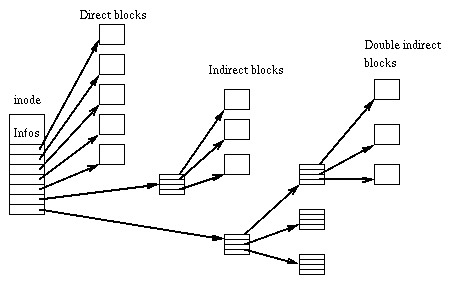
\includegraphics{Ext2-inode.jpg}
\end{center}

Luego un sistema de archivos será un conjunto (una tabla) de estos
nodos-i (estructuras) guardados dentro de la partición que contiene el 
sistema de archivos. 

\fcolorbox{black}{grey}{
\parbox[t]{1.0\linewidth}{ \vspace*{0.4cm}
{\bf 
Una conclusión que puede derivarse, es que 
el sistema de archivos en sí mismo consume espacio para almacenar las 
estructuras dentro del dispositivo de almacenamiento, lo cual debe ser 
tenido en cuenta a la hora de diseñar el tamaño del sistema de archivos. 
}
\vspace*{0.4cm} } }


\subsection*{Sistemas de archivos soportados por Linux}

Linux soporta una gran cantidad de tipos diferentes de sistemas de archivos.Con soportar nos podemos estar refiriendo a lectura y escritura, o en 
algunos casos sólo lectura. Para nuestros propósitos los más importantes 
son:

{\bf ext4 (fourth extended filesystem o «cuarto sistema de archivos 
extendido»)}

Es un sistema de archivos transaccional (en inglés journaling), anunciado 
el 10 de octubre de 2006 por Andrew Morton, como una mejora compatible de 
ext3. Esto significa que es posible montar un sistema de archivos ext3 como
ext4 y usarlo transparentemente, mientras que la reversa puede no ser 
siempre válida. Es la versión utilizada en la mayoría de los sistemas Linux
modernos. 

{\bf ext3}

    El sistema de archivos ext3 posee todas las propiedades del sistema de
archivos ext2. La diferencia es que se ha añadido una bitácora (journaling).
Esto mejora el rendimiento y el tiempo de recuperación en el caso de una 
caída del sistema y consecuente corrupción del sistema de archivos. 
Actualmente aún muy utilizado. 

{\bf ext2}

La principal desventaja de ext2 es que no implementa la bitácora (en inglés
Journaling) que sí poseen sus posteriores versiones ext3 y ext4. ext2 fue 
el sistema de archivos predeterminado de las distribuciones GNU/Linux Red 
Hat, Fedora Core y Debian. Los lanzamientos de las nuevas versiones 
estables, ext3 y ext4, han desplazado considerablemente su uso. Está 
diseñado para ser compatible con diseños futuros, así que las nuevas 
versiones del código del sistema de archivos no  necesitan rehacer los 
sistemas de archivos existentes.

{\bf reiserfs}

    Un sistema de archivos robusto. Se utiliza una bitácora que provoca
que la pérdida de datos sea menos frecuente. La bitácora es un mecanismo 
que lleva un registro por cada transacción que se va a realizar, o que ha 
sido realizada. Esto permite al sistema de archivos reconstruirse por sí 
sólo fácilmente tras un daño ocasionado, por ejemplo, por cierres del 
sistema inadecuados. 

{\bf XFS  }

XFS es un sistema de archivos de 64 bits con journaling de alto rendimiento
creado por SGI (antiguamente Silicon Graphics Inc.) para su implementación 
de UNIX llamada IRIX. En mayo de 2000, SGI liberó XFS bajo una licencia de 
código abierto. 

XFS se incorporó a Linux a partir de la versión 2.4.25. Los programas de 
instalación de las distribuciones de SuSE, Gentoo, Mandriva, Slackware, 
Fedora Core, Ubuntu y Debian ofrecen XFS como un sistema de archivos más.

Esta diseñado para archivos y sistemas de archivos de gran tamaño.

Por cuestiones de interoperabilidad, se hace necesario en muchos casos
poder leer o escribir sobre sistemas de archivos que no son nativos de 
GNU/Linux. Por este motivo, existe soporte para sistemas de archivos 
adicionales, nativos de otros sistemas operativos o productos privativos. 
De este modo, se facilita el intercambio de archivos con otros sistemas 
operativos. 

Desde el punto de vista de un usuario, estos sistemas de archivos ajenos 
funcionan exactamente como los nativos, sin embargo pueden carecer de 
algunas características. Por ejemplo el sistema de archivos vxfs (propiedad
de Symantec) tiene soporte en Linux que permite que estos sistemas de 
archivos sean leído pero no escritos. 

Algunos de los sistemas de archivos, no nativos, de interés son: 

{\bf ntfs} 
    Compatibilidad con el sistema de archivos NTFS de Microsoft Windows. 
Permite lectura y escritura. 

{\bf msdos}

    Compatibilidad con el sistema de archivos FAT de MS-DOS (y OS/2 y Windows NT).

{\bf umsdos}

    Extiende el dispositivo de sistema de archivos msdos en Linux para obtener nombres de archivo largos, propietarios, permisos, enlaces, y archivos de dispositivo. Esto permite que un sistema de archivos msdos normal pueda utilizarse como si fuera de Linux, eliminando por tanto la necesidad de una partición independiente para Linux.

{\bf vfat}

    Esta es una extensión del sistema de archivos FAT conocida como FAT32. Soporta tamaños de discos mayores que FAT. La mayoría de discos con MS Windows son vfat.

{\bf iso9660}

    El sistema de archivos estándar del CD-ROM; la extensión popular Rock Ridge del estándar del CD-ROM que permite nombres de archivo más largos se soporta de forma automática.

{\bf NFS (Network File System)}

    Un sistema de archivos de red que permite compartir un sistema de archivos entre varios ordenadores para permitir fácil acceso a los archivos de todos ellos.

{\bf smbfs (SAMBA file system)}

    Un sistema de archivos que permite compartir un sistema de archivos con
un ordenador MS Windows a través de la red. Es compatible con los 
protocolos para compartir archivos de Windows. 


Existen también otros sistemas de archivos creados y utilizados por el 
sistema operativo en sí mismo. Este es el caso del sistema de archivos 
\texttt{proc}, generalmente accesible desde el directorio /proc, que en 
realidad no es un sistema de archivos, aún cuando lo parece. El sistema 
de archivos proc 
facilita acceder a ciertas estructura de datos del núcleo, como la lista 
de procesos (de ahí el nombre). Hace que estas estructuras de datos 
parezcan un sistema de archivos, y que el sistema de archivos pueda ser 
manipulado con las herramientas de archivos habituales. Por ejemplo, para
obtener una lista de todos los procesos se podría utilizar el comando 
\texttt{ls -ld /proc/[0-9]*}, cada directorio numérico se corresponde con
un PID. 


\subsection*{¿Qué sistemas de archivos deben utilizarse?}

No existe un regla que establezca la mejor opción parar todos los casos. 
La elección del sistema de archivos a utilizar depende de la situación. Si 
la compatibilidad o alguna otra razón hace necesario uno de los sistemas 
de archivos no nativos, entonces hay que utilizar ése. Si se puede elegir 
libremente, entonces lo más recomendable sería utilizar ext4, ya que es 
la opción predeterminada y nativa. 

Existe generalmente poca ventaja en utilizar muchos sistemas de archivos 
distintos en una misma computadora. Actualmente, el más popular 
sistema de archivos en las distribuciones GNU/Linux es ext4, debido a que 
es un sistema de archivos con bitácora. Sin embargo, podríamos necesitar 
un sistema de archivos diseñado para archivos grandes, en cuyo caso 
el sistema de archivos xfs podría ser una elección. Cada caso debe ser
analizado previo a realizar una elección.

\subsection*{Crear un sistema de archivos}

Un sistema de archivos se crea, esto es, se crean y guardan en el disco las
estructuras de datos lógicas que permiten la organización de los archivos,
con el comando \texttt{mkfs}. Existen en realidad programas separados para 
cada tipo de sistemas de archivos. \texttt{mkfs} es únicamente una careta 
que ejecuta el programa apropiado dependiendo del tipo de sistemas de 
archivos deseado. El tipo se selecciona 
con la opción ``\texttt{-t fstype}''. Es así que si creamos ejecutamos 
el comando \texttt{mkfs -t vfat}, en realidad terminaremos invocando 
el comando \texttt{mkfs.vfat}.

Los programas a los que ``\texttt{-t fstype}'' invoca tienen líneas de 
comando ligeramente diferentes dependiendo de las características 
particulares del sistema de archivos a construir. En algunos casos 
puede ser necesario cambiar los valores predeterminados, por lo que 
recurriremos a la página del manual correspondiente al comando específico 
para la construcción del sistema de archivos en cuestión, por ejemplo 
``\texttt{man mkfs.vfat}''.  


\colorbox{grey}{\parbox[t]{0.95\linewidth}{ \vspace*{0.5cm} { 
{\bf Ejemplo: crear sistema de archivos ext3 en /dev/sdc1 }\\
{\tt
\# mkfs -t ext3 /dev/sdc1\\
mke2fs 1.42.8 (20-Jun-2013)\\
Etiqueta del sistema de ficheros=\\
OS type: Linux\\
Tamaño del bloque=4096 (bitácora=2)\\
Tamaño del fragmento=4096 (bitácora=2)\\
Stride=0 blocks, Stripe width=0 blocks\\
65536 inodes, 262144 blocks\\
13107 blocks (5.00\%) reserved for the super user\\
Primer bloque de datos=0\\
Número máximo de bloques del sistema de ficheros=268435456\\
8 bloque de grupos\\
32768 bloques por grupo, 32768 fragmentos por grupo\\
8192 nodos-i por grupo\\
Respaldo del superbloque guardado en los bloques: \\
	32768, 98304, 163840, 229376\\
\\
Allocating group tables: 0/8   hecho                           \\
Escribiendo las tablas de nodos-i: 0/8 hecho                           \\
Creating journal (8192 blocks): hecho\\
Escribiendo superbloques y la información contable del sisteDel comando anterior observamos que todos los PID listados pertenecen al 
usuario lechnerm. Una opción será entonces comunicarse con el usuario y 
pedirle que cierre sus programas amablemente. }
} \vspace*{0.5cm} } } 

\subsection*{Montar y desmontar sistemas de archivos}

Antes de que se pueda utilizar un sistema de archivos, debe ser montado. 
Durante este proceso el sistema operativo realiza operaciones de 
mantenimiento para asegurarse que todo funciona correctamente. 
Como todos los archivos en UNIX están en un mismo árbol, independizando 
al usuario de la ubicación física real de cada archivo, la operación de 
montaje provocará que el contenido del nuevo sistema de archivos 
aparezca como dentro de un subdirectorio existente en algún 
sistema de archivos montado previamente.

Por ejemplo, es usual que el subdirectorio \texttt{/home} tenga su propio 
sistema de archivos en una partición separada del sistema de archivo raíz.
En este caso, si el sistema de archivos de \texttt{/home} no se encuentra
montado, al listar el directorio observaremos que su contenido 
esta vació. Luego, al montar la partición de disco que contiene el sistema
de archivos de \texttt{/home}, hacemos visible su contenido, es decir que 
al listar el contenido de \texttt{/home} obtendremos la lista de archivos
guardados en esa partición. 

El directorio dónde se ``engancha'' o monta el sistema de archivos se 
conoce como ``\textit{punto de montaje}''. Por ejemplo, diremos que el 
dispositivo {/dev/sda2} se encuentra montado en el punto de montaje 
\texttt{/home}. De este modo, los puntos de montajes son subdirectorios, 
que comienzan a partir del directorio raíz y es donde se presentan los
sistemas de archivos almacenados en los dispositivos, para su acceso.  

Los comando \texttt{mount} y \texttt{umount} permiten montar y desmontar
respectivamente sistemas de archivos. 

\textbf{El comando \texttt{mount}}

El comando mount permite entre otras cosas, listar los sistemas de 
archivos actualmente montados y sus propiedades de montaje. Por ejemplo: 


\colorbox{grey}{\parbox[t]{0.95\linewidth}{ \vspace*{0.5cm} { 
{\bf Ejemplo: salida del comando \texttt{mount}} \\ 
{\tt
\# mount\\ 
sysfs on /sys type sysfs (rw,nosuid,nodev,noexec,relatime)\\
proc on /proc type proc (rw,nosuid,nodev,noexec,relatime)\\
udev on /dev type devtmpfs (rw,relatime,size=10240k,nr\_inodes=946053,mode=755)\\
tmpfs on /run type tmpfs (rw,nosuid,noexec,relatime,size=758272k,mode=755)\\
/dev/sda1 on / type ext4 (rw,relatime,errors=remount-ro,data=ordered)\\
/dev/sda2 on /home type ext4 (rw,relatime,errors=remount-ro,data=ordered)\\
nodo3:/mnt/500gb on /mnt type nfs (rw,relatime,vers=3,rsize=262144,\\ 
wsize=262144,namlen=255,hard,proto=tcp,timeo=600,retrans=2,sec=sys,\\ 
mountaddr=192.168.0.33,mountvers=3,mountport=56384,mountproto=udp,\\
local\_lock=none,addr=192.168.0.33)\\
\\
}
} \vspace*{0.5cm} } } 

El comando mount, también nos permite montar nuevos sistemas de archivos 
dentro de la jerarquía de directorios. Para este caso, recibe dos 
argumentos. El primero es el archivo de 
dispositivo correspondiente al disco o partición que contiene el sistema 
de archivos. El segundo es el directorio bajo el cual va a ser montado. 

\colorbox{grey}{\parbox[t]{0.95\linewidth}{ \vspace*{0.5cm} { 
{\bf Ejemplo:} \\
{\tt
\# mount /dev/sda2 /usr\\
\# mount /dev/sdb2 /home\\ 
}
} \vspace*{0.5cm} } } 

Tras estos dos comandos el contenido de los dos sistemas de archivos 
aparecen como los contenidos de los directorios /home y /usr, 
respectivamente. Se dice que ``/dev/sdb2 está montado en /home'', e 
igualmente para /usr, ``/dev/sda2 está montado en /usr''. Para ver
cualquiera de los sistemas de archivos, se puede mirar el contenido del 
directorio en el que fue montado, como si fuera cualquier otro directorio.

Observe la diferencia entre el archivos de dispositivo, /dev/sda2, y el 
punto de montaje, /home. El archivo de dispositivo proporciona acceso al 
contenido crudo del disco, el directorio de montaje proporciona acceso a 
los archivos del disco. El directorio de montaje se denomina punto de 
montaje.

Linux soporta multitud de sistemas de archivos, el comando \texttt{mount}
intentará adivinar el tipo de sistema de archivos. Se puede utilizar 
la opción ``\texttt{-t fstype}'' para especificar el tipo manualmente; 
esto es necesario en determinados casos, puesto que la heurística que 
utiliza \texttt{mount} no siempre funciona. Por ejemplo, para montar
un disco MS-DOS, se puede utilizar el comando siguiente:

\colorbox{grey}{\parbox[t]{0.95\linewidth}{ \vspace*{0.5cm} { 
{\tt
\# mount -t msdos /dev/sdc1 /mnt
}
} \vspace*{0.5cm} } } 

El directorio de montaje deberá estar vacío, aunque debe existir. 
Cualquier archivo existente en él, en cualquier caso, será inaccesible 
por su nombre mientras el nuevo sistema de archivos esté montado 
(quedará oculto bajo el nuevo sistema de archivos montado. Cualquier 
archivo que estuviera abierto seguirá estando accesible). 

El comando mount también permite especificar ciertas opciones acerca del 
sistema de archivos a montar. Por ejemplo, si no tiene intención de 
escribir nada en el sistema de archivos a montar, puede utilizar la 
opción  \texttt{-r} de mount para realizar un montaje de sólo lectura. 
Esto provocará que el núcleo detenga cualquier intento de escribir en el 
sistema de archivos, y también impedirá que el núcleo actualice el tiempo 
de acceso a los nodos-i.

El lector atento habrá notado un ligero problema lógico. ¿Cómo se monta 
el primer sistema de archivos (denominado sistema de archivos raíz, ya que 
contiene al directorio raíz), si obviamente no puede montarse sobre otro 
sistema de archivos? Bueno, la respuesta es que se realiza un truco de
 magia. El sistema de archivos raíz se monta mágicamente a la hora 
del arranque, y se puede confiar en que siempre será montado. Si el 
sistema de archivos no puede montarse, el sistema no arrancará. El 
nombre del sistema de archivos que mágicamente se monta como root está 
compilado dentro del núcleo, o se especifica utilizando opciones del gestor
de arranque.

En muchos sistemas existen otros sistemas de archivos que también deben 
montarse de forma automática durante en el arranque. Estos se especifican 
en el archivo de configuración \texttt{/etc/fstab} ; 
vea la página de manual de fstab para los 
detalles en el formato. Los detalles sobre cuándo se montan exactamente 
los sistemas de archivos adicionales dependen de muchos factores, y 
pueden ser configurados por cada administrador si lo necesita.

\textbf{El comando \texttt{umount}}

Cuando un sistema de archivos no necesita seguir montado, puede 
desmontarse con el comando  \texttt{umount}. Dicho comando toma un 
argumento: o bien el archivo de dispositivo o el punto de montaje. 
Por ejemplo, para desmontar los directorios del ejemplo anterior, 
se pueden utilizar los comandos: 

\colorbox{grey}{\parbox[t]{0.95\linewidth}{ \vspace*{0.5cm} { 
{\bf Ejemplo:} \\
{\tt
\# umount /usr\\
\# umount /dev/sdb2\\ 
}
} \vspace*{0.5cm} } } 

Debido al buffer cache de disco, los datos no se escriben necesariamente 
hasta que se desmonta el sistema de archivos. De modo que remover un 
dispositivo de almacenamiento sin cuidado, puede provocar 
errores en el contenido del sistema de archivos. \textbf{El comando 
\texttt{umount}} garantiza que todos las escrituras pendientes, se 
reflejen en el disco antes de desmontar el sistema de archivos, 
garantizando que todos los datos y estructuras del sistema de archivos 
se encuentren en buen estado.

\fcolorbox{black}{grey}{
\parbox[t]{1.0\linewidth}{ \vspace*{0.4cm}
{\bf Lo importante:}  en el caso de dispositivos removibles en caliente, 
como una memoria flash usb, es de suma importancia desmontar los sistemas
de archivos que hubiera montados \textbf{antes} de desconectar el
dispositivo. La omisión de este paso puede involucrar pérdida de datos 
dentro del sistema de archivos.  
\vspace*{0.4cm} } }

También es importante notar que para poder desmontar un sistema de archivos,
el mismo no debe estar en uso. Esto significa que ningún proceso debe
tener archivos abiertos que se encuentren en el sistema de archivos a
desmontar. Si intentamos desmontar un sistema de archivos en uso, el 
comando \texttt{umount} fallará. En este caso, el administrador deberá 
averiguar cuáles son los procesos y archivos abiertos. Los comandos 
\texttt{fuser} y \texttt{lsof} son de gran utilidad a la hora de averiguar 
esta información.   


\colorbox{grey}{\parbox[t]{0.95\linewidth}{ \vspace*{0.5cm} { 
{\bf Ejemplo de detección de archivos abiertos: } \\
{\tt
\# fuser -cu /home \\ 
/home:                2967cm(lechnerm)  3012m(lechnerm)  3023cm(lechnerm) \\
 3038m(lechnerm)  3060cm(lechnerm)  3064cm(lechnerm)  3109cm(lechnerm) \\ 
3111c(lechnerm)  3114c(lechnerm)  3116c(lechnerm)  3119c(lechnerm)  \\
}
Del comando anterior observamos que todos los PID listados pertenecen al 
usuario lechnerm. Una opción será entonces comunicarse con el usuario y 
pedirle que cierre sus programas amablemente. 
} \vspace*{0.5cm} } } 



Montar y desmontar requieren privilegios de superusuario, esto es, sólo 
root puede hacerlo. La manipulación incorrecta, intencional o no, del 
sistema de archivos puede dañar seriamente el funcionamiento del sistema. 
Por ejemplo un usuario desprevenido podría desmontar el sistema de archivos
montado en /home y causar que el resto de los usuarios no puedan acceder 
a sus datos, o ingresar al sistema. Esta restricción puede resultar 
incómoda, cuando hablamos de sistemas de archivos en dispositivos
removibles, como un pendrive. Para solucionar el problema, se usan 
diversos métodos, entre ellos la manipulación de grupos y permisos sobre 
los archivos de dispositivo particulares. 

\section*{Licencia}
This is a derived version of "Guía Para Administradores de Sistemas GNU/Linux" that 
can be found at \\ \texttt{http://www.ibiblio.org/pub/Linux/docs/LDP/system-admin-guide/translations/es/gasl.txt}.

Copyright (C) 1993-1998 Lars Wirzenius.

Copyright (C) 1998-2001 Joanna Oja.

Copyright (C) 2001-2003 Stephen Stafford.

Copyright (C) 2003-2004 Stephen Stafford and Alex Weeks.

Copyright (C) 2004-Present Alex Weeks.

Copyright (C) 2013-Present Rafael Ignacio Zurita

Trademarks are owned by their owners.

Permission is granted to copy, distribute and/or modify this document under
the terms of the GNU Free Documentation License, Version 1.2 or any later
version published by the Free Software Foundation; with no Invariant
Sections, no Front-Cover Texts, and no Back-Cover Texts. A copy of the
license is included in the section entitled "GNU Free Documentation License".

\subsection*{Traducción de la licencia}
Esta es una obra derivada de "Guía Para Administradores de Sistemas GNU/Linux" que puede 
econtrarse en \\ \texttt{http://www.ibiblio.org/pub/Linux/docs/LDP/system-admin-guide/translations/es/gasl.txt}.

Las marcas registradas son propiedad de sus dueños.

Se concede autorización para copiar, distribuir y/o modificar este documento
bajo los términos de la Licencia de documentación libre GNU (FDL), Versión 1.2; 
sin Secciones Invariantes, sin textos de Portada, y sin Textos de Contra Portada. 
Una copia de la licencia se encuentra incluída en la sección "GNU Free Documentation License".


\end{document}
